% 卒論向けLaTex用テンプレート
% by Toshiya Sasaki
% http://www.math.tohoku.ac.jp/~atsushi/Tex/index.htmlよりmysect.styを使用しています.
\AtBeginDvi{\special{pdf:mapfile motoya.map}} %コンパイル時に強制的にmapファイルを使用する設定

\documentclass[titlepage,a4paper,11pt]{jreport}
\title{タイトル}
\author{情報電子工学系学科 複雑数理モデル研究室\\おなまえ かいてね}
\date{--年--月--日}

%\usepackage[dvipdfmx,colorlinks=false,bookmarks=true,bookmarksnumbered=false,pdfborder={0 0 0},bookmarkstype=toc]{hyperref}



\usepackage[dvipdfmx]{graphicx}
\usepackage{amsmath}
\usepackage{calc,fancybox}
\usepackage{mysect}
\usepackage{url}
\usepackage{here}
\usepackage{subcaption}


%行間を倍にする 校正時に使用
%\renewcommand{\baselinestretch}{2}


%fverbatimを定義する.
%verbatimの改造版,外枠をつけられる.
\newenvironment{fverbatim}[1]%
{\VerbatimEnvironment
\begin{Sbox} \begin{minipage}{#1}%
\begin{Verbatim}}{\end{Verbatim}%
\end{minipage}\end{Sbox}%
\fbox{\TheSbox}}

%マージン・参考文献タイトル等の書式設定
\numberwithin{equation}{chapter}
\renewcommand{\bibname}{参考文献}
\setlength{\oddsidemargin}{25mm} % 奇数ページ 左マージン 10mm
\addtolength{\oddsidemargin}{-1in}% 奇数ページ 標準のマージン(1inch)を引く
\setlength{\evensidemargin}{25mm}% 偶数ページ 左マージン 10mm
\addtolength{\evensidemargin}{-1in} % 偶数ページ 標準のマージン(1inch)を引く
\setlength{\textwidth}{160mm} %本文の長さ(横) 210 -(30+15) = 165


\begin{document}
%表紙・目次の表示
\maketitle 
\tableofcontents

%図目次
\newpage
\listoffigures

%表目次
\newpage
\listoftables

\newpage

\chapter*{概要}
これは概要である.chapter*とすることで章番号をつけることなく見出しにすることができる.必要に応じて使うが,概要と付録にしか使わない.\par
付録か過去のものをそのまま使用している.必要に応じて参考にすること.なお,ページ番号等目次の反映にはコンパイルが2回必要なことが多いことに注意する.

% !TEX root = ../main.tex
\chapter{はじめに}

\section{背景}
この文章は論文テンプレートである.作成者は大園 章宏(15024025/19043014)なので何かあれば適当にwikiの個人ページをのぞくと良いが,特に有益な情報は載せていないことに注意したい.\par
論文の構成は書いた後に入れ替えることが多いため,各項目をinputする形で使用したい.


%文末
\clearpage



\begin{thebibliography}{99}
\addcontentsline{toc}{chapter}{\bibname}% タイトル追加
\bibitem{a} 浅田稔,國吉康夫,ロボットインテリジェンス,(2006)
\end{thebibliography}


% 付録を目次に追加
\clearpage 
\addcontentsline{toc}{chapter}{付録} 


\appendix
\def\appendixsymbol{付録}
\section{付録とは}
付録とは本や雑誌などについてくるおまけのようなもののことである.

\subsection{サブセクション}
サブセクションも使えると考えれる。


\newpage
\section{画像}
画像(がぞう)は、2次元平面上に描かれた絵を指す。
画像には静止画(静止画像)と動画(動画像)とがあるが
動画像は映像と呼ばれることが多く、この項目では静止画像について記述する。
コンピュータ上の静止画像はデジタルカメラの写真や、コンピュータグラフィックスなどから生成されたものがあり、自動的、半自動的な画像処理や画像認識に向くという特徴がある。

\begin{figure}[htbp]
\begin{center}
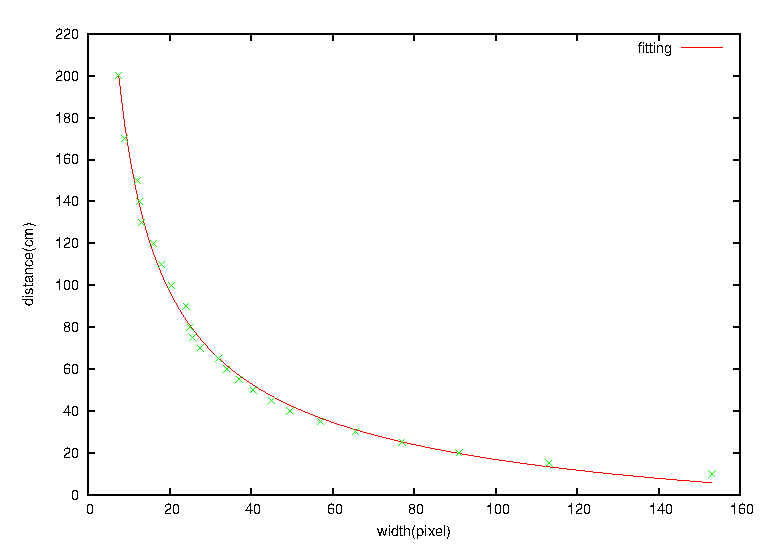
\includegraphics[width=0.5\linewidth]{appendix/eps/pixy.eps}
\caption{XXXXの画像}
\label{ラベルの名前}
\end{center}
\end{figure}

\newpage

\section{表}
表は、ビジュアルコミュニケーションの一形態であり、データを並べる手段である。
テーブルはコミュニケーション、研究、データ解析など様々な分野で使われている。
印刷物、手書きのノート、コンピュータソフトウェア、建築装飾、交通標識など様々なところでテーブルを見つけることができる。
\begin{table}[htbp]
\caption{XXXXの表}
\begin{center}
\begin{tabular}{|cl|}
\hline
主翼幅 & 880[mm] \\
主翼面積 & 1325[cm$^2$] \\
平均翼弦& 150[mm] \\
水平尾翼面積 & 267[cm$^2$] \\
モーメントアーム長 & 500[mm] \\
水平尾翼容積 & 0.67[-] \\
重心位置 & 75[mm] \\
         & (平均翼弦の50\%) \\
機長 & 840[mm] \\
機体重量 & 470[g] \\
(バッテリー含む) &  \\
\hline
\end{tabular}
\end{center}
\end{table}

\newpage

\section{fverbatimの例}
fverbatimをfigureで囲むことで図として扱っている.

\begin{figure}[htbp]
\begin{fverbatim}{1.1\linewidth}
◎ [armadillo300 ~]# fdisk /dev/hda
hda: hda1
◎ Command (m for help): d
Selected partition 1
◎ Command (m for help): n
Command action
   e extended
   p primary partition (1-4)
◎ p
\end{fverbatim}
\caption{コマンド手順1}
\label{ラベル名}
\end{figure}



\end{document}
